% LLNCStmpl.tex
% Template file to use for LLNCS papers prepared in LaTeX
%websites for more information: http://www.springer.com
%http://www.springer.com/lncs

\documentclass{llncs}
%Use this line instead if you want to use running heads (i.e. headers on each page):
%\documentclass[runningheads]{llncs}

\usepackage{graphicx}
\usepackage{enumitem}

\graphicspath{ {Figures/} }

\newlist{hypotheses}{enumerate}{1}
\setlist[hypotheses]{label=\textbf{H\arabic*:}}


\begin{document}
\title{Document Classification}

%If you're using runningheads you can add an abbreviated title for the running head on odd pages using the following
%\titlerunning{abbreviated title goes here}
%and an alternative title for the table of contents:
%\toctitle{table of contents title}

\subtitle{Applied Natural Language Processing \\ Coursework 1}

%For a single author
\author{Paul-Michael Sorhaindo - 119875}

%For multiple authors:
%\author{Paul-Michael Sorhaindo\inst{1}}


%If using runnningheads you can abbreviate the author name on even pages:
%\authorrunning{abbreviated author name}
%and you can change the author name in the table of contents
%\tocauthor{enhanced author name}

%For a single institute
%\institute{Institute Name \email{email address}}

% If authors are from different institutes 
\institute{University of Sussex \email{ps324@sussex.ac.uk}}

%to remove your email just remove '\email{email address}'
% you can also remove the thanks footnote by removing '\thanks{Thank you to...}'


\maketitle

\begin{abstract}
This paper conducts a few experiments in document classification looking at the speculative word list classifier, derived word list classifier and the Na\"\i ve Bayes classifier. These document classifiers are used for the purpose of sentiment analysis in order to correctly predict the sentiment, either positive or negative, of the document. The experiments look at both comparing the classifiers accuracy as well as attempting to improve them.
\end{abstract}

\section{Introduction}
Document classification is an area of Natural Language Processing in which algorithms are produced that given a document will assign it to a category. The categories that documents are assigned to vary depending on the type of document classification task being performed. Sometimes these categories may be topics or themes, in the case of a topic relevance tester, or in the case of document filters, the categories could be simply accepted or not accepted. This paper will look at sentiment analysis, another form of document classification, which is used to determine whether documents presenting a subject in a positive or negative light.

The aim of this paper is to explore different document classification methods and produce quantifiable evidence as to which methods are more effective. Furthermore the experiments will look at the effects of using different methods of training and providing data to such classifiers. Methods of splitting the sample data used for development and testing within the experiments will also be analysed.

\section{Types of Classifier}
There are several approaches to producing a document classifier, the following section will look at three of them and endeavour to explain how they make their conclusions about a given document's classification. 

\subsection{Speculative Word List Classifier}
Word list classifiers work on an assumption that the presence of a word within a document of a particular category is indicative of the fact that the document belongs to that particular category. In a speculative word list classifier, word lists are compiled for each category by the developer. These are based on both their own knowledge and intuition of the categories within which the documents are to be classified. The classification algorithm works by getting a frequency for each word's occurrence within the document when it is on the speculative word list. The frequencies of the words in each category’s word list are then then summed to produce a score for the document in that category. These scores would  then be compared with the category whose word list frequency summation score is the highest, the category with the highest score is put forward as the classification result. A variable can also be added to this algorithm in the form of a margin, that the difference between the two category scores must be greater than, in order for the document to be classified as belonging to either one category or the other. 

% TODO Has the advantage of not needing tagged data.
% Disadvantage humans have different ways of formulating their views through language and one person’s point of view may not be an accurate representation of constitutes important words for the classification task at hand.

\subsection{Derived Word List Classifier}
The difference between the derived word list classifier and the speculative word list classifier is the method through which the word list for each category is produced. In order to derive these word lists automatically labelled sample documents need to be provided for training. The classifier is then tested and evaluated on data that is separate from the sample data. One method of choosing words for a category's word list is to simply take the most frequently occurring terms used throughout all documents with the same label. Another method looks at the amount of times a term frequency within the sample data of a category and subtracts the amount of times the term occurs in documents which aren't labelled as the same category. Terms that score high in this method not only occur frequently in their category but are also less frequently used in other categories.
% TODO The amount of words that are included in the derived words can be adjusted, and say why!

\subsection{Na\"\i ve Bayes Classifier}
Akin to the derived word list the Na\"\i ve Bayes approach to document classification involves utilising a sample set of documents in order for the classifier to be trained. The algorithm looks at the probability of each term occurring within a particular classification of documents. Bayes' theorem is then applied.

\begin{equation}
    \Pr(A|B)=\frac{\Pr(B|A)\Pr(A)}{\Pr(B)}
\end{equation}

This gives us a way to calculate the probability of A given B which can be used for classification of documents. The training data set is analysed by the classifier and probability for each term occurring within the labelled training data of a particular classification is calculated. The probabilities are compared to the probabilities of terms occurring within the testing data to be classified the terms that do not appear within the training are provided through Laplace smoothing, by adding an extra occurrence for all terms that appeared during the training of the classifier as well as the new terms within the document to be classified. The product of all the probabilities that the document to be classified is a particular classification given that it contains a term is calculated. Once these products are computed for each classification the classification with the highest probability is chosen for the document.

\section{Aim}
This paper aims to compare the different document classifiers that have been discussed when used for the purpose of sentiment analysis. Experiments will be performed using these classifiers on the labelled Amazon Review corpus. The classifiers will be trained or configured as necessary on training data before being tested by classifying previously unseen documents as either carrying a positive or negative sentiment. The effect of varying the amount of training and testing data, as well as the varying of subject matter for training and testing will also be explored.

\section{Hypotheses} % TODO ensure all hypotheses are linked to.
\label{sec:hypotheses}
The following hypotheses are put forward:

\begin{hypotheses}
    \item \label{hyp:h1} When comparing a speculative word list classifier used to determine whether a document is either positive or negative with a tuned derived word list, the derived word list classifier will produce a value of accuracy greater than or equal to that of the speculative word list classifier.
    
    \item \label{hyp:h2} The Na\"\i ve Bayes classifier will produce a better accuracy than derived word list, when the training set is a large sample of training data.
    
    \item \label{hyp:h3} The accuracy of the NB Classifier will increase as the training data set increases.
    
    \item \label{hyp:h4} When testing a Na\"\i ve Bayes classifier which has only been trained on one type of review for example book reviews it will do significantly better on testing data comprised of only of book reviews.
    
    \item \label{hyp:h5} The results for the accuracy of the Na\"\i ve Bayes will improve when certain features are removed from the training and testing data sets. Specifically when the difference between lowercase and uppercase characters is ignored, numbers are removed from the data sets and stop words a filtered.
\end{hypotheses}

\section{Methodology}

The hypotheses proposed in the previous section will be tested by carrying out several practical experiments on the implementations of the three document classification algorithms described above. The provided Amazon Review corpus will be randomly split into training and validation data with 80\% of the data been set aside for training and 20\% for testing. The classifier being tested is then trained on the training data, and its classification accuracy measured using the testing data with the mean average result over the splits being taken as the classifiers result. The size of word lists, where used, and the changes in accuracy that varying this size produces, will be explored through experimentation. Further experiments will keep the size of the word lists uniform to ensure consistency when making comparisons.

\subsection{Word List Based Approaches}
The first tests will take place on the speculative word list classifier the results of which will form as reference for future tests. The classifier will be given random sub samples of the Amazon Review corpus and its accuracy will be measured over thirty trails where a random 80:20 split of the data set between training and testing data is taken. The positive and negative word lists used are purely speculative and based on what the author believed to be words which would likely give a document a positive or negative sentiment.

After these results have been documented, experiments will be performed on derived word list approaches and the effect of changing different hyper parameters, the best result being taken forward for a comparison to be made between the derived and speculative word list approaches.

\subsection{Na\"\i ve Bayes Approach}
Tests on the Na\"\i ve Bayes Classifier (implementation provided by the NLTK library) will take place in the same conditions as the speculative and improved derived word list classifier tests. This will allow a comparison of a Na\"\i ve Bayes method of document classification with word list and score based approaches.

\subsubsection{Varying Training Data Size}
Next the size of the training data used to train the Na\"\i ve Bayes Classifier will be varied to gauge the effect of reducing the size of the algorithm's training data set on the accuracy of its classification process. The experiment will take four different sizes of training data and compare them using a fixed size testing set.

\subsubsection{Changing feature extraction methods}
Data in the corpus can be formatted before being trained on. This may improve the classifiers performance when training on a set of training data. To determine whether or not extracting particular features from the text will improve the Na\"\i ve Bayes Classifier three experiments will be performed using compounding feature extraction techniques. The effects in the average accuracy over the thirty trails will be compared to monitor the effects that feature extraction has on the accuracy of the classifier.

\subsubsection{Changing Domain}
As the Amazon Review corpus is divided into several domains (reviews on books, electronics, DVD's and kitchen items). Experiments will take place in order to determine whether or not the subject of a review affects a classifier when it is trained on reviews of one subject and then tested on a different subject. In order to carry out these experiments classifiers are trained on each domain against a particular domain for a single round of thirty tests. 

\subsubsection{Most Informative Features Comparison}
The NLTK library provides the function show\textunderscore most\textunderscore informative\textunderscore features() which returns a list of the `most informative' features used by the classifier.
The NLTK documentation defines the informativeness of a feature as equal to the highest probability for a feature, divided by the lowest probability for any feature. This list contains the words which are most influential in classifying documents using the Na\"\i ve Bayes Classifier model. This list of words will be compared with the words that the derived word list approach chose in order to score documents during classification and also with the speculative wordlist that was put together by the author.

\section{Implementation}
The Python code that the experiments run on is organised into five modules; nle\textunderscore utils.py contains an extensive list of helper functions which assist in manipulating the data between certain forms in order to be in the correct structure for the other functions provided by the Natural Language Toolkit (NLTK) and the University of Sussex, this module also contains two hardcoded arrays for the speculative word lists.

The simple\textunderscore classifier.py module consists of a class which implements the frequency and score based classifier used by both the speculative and derived word list approaches. This class is instantiated in the file simple\textunderscore classifier\textunderscore testing.py, the contents of which form a script which details the process of experiments performed using score based classifiers. The naive\textunderscore bayes\textunderscore testing.py script is structured similarly to simple classifier's script both scripts use a global variable called feature\textunderscore extractor which is assigned a function. This partial function is passed on as a parameter to helper functions which format the training and testing data by removing features from the data that the functions specify. The value None can be passed through instead of a function to leave the text unformatted.

The final script used in the experiments is results.py. This code allows the text files produced by the \textunderscore testing.py scripts which contain the all the values produced by a single experiment. These values are read in and parsed back into python data structures which can then be used to display graphs with the help of the NumPy and matplotlib python libraries.

\section{Results and Analysis}
The following section presents the results of the experiments detailed in the methodology, these results will be discussed, with patterns or anomalies being highlighted and where possible explanations for their occurrence. References will also be made to the hypotheses put forward in ~\ref{sec:hypotheses} to show whether or not they have been refuted.

\subsection{The Three Classifiers}

In first few experiments the accuracy of the Specified word list and Derived wordlist classifiers are tested as well as the Na\"\i ve Bayes Classifier. These tests took place on a domain specific basis, so that the classifiers were trained on the domains that they were tested on. The tests results are the mean value of thirty trials and the average of these results and their standard deviation is tabulated in Table~\ref{tab:three_classifiers_table}.

\begin{table}
    \begin{center}
    \caption{The mean accuracies for each type of classifier compared.}
    \label{tab:three_classifiers_table}
    \begin{tabular}{| l | l | l |}
        \hline
        Feature Extractor & Mean Accuracy & Std. Deviation \\ \hline
        Speculative Classifier & 0.5956 & 0.01663 \\ \hline
        Derived Classifier & 0.6304 & 0.01915 \\ \hline
        Na\"\i ve Bayes Classifier & 0.7811 & 0.0319 \\ \hline
    \end{tabular}
    \end{center}
\end{table}


The means were computed across domain specific experiments on separate results in the Python console. An interesting anomaly was the accuracy produced by the Speculative word list approach for the DVD domain which resulted in an accuracy of 0.6241 where other domains only produced an accuracy of 0.58 (to two significant figures) This could indicate that the speculative word list produced by the author is more suited to DVD review classification than other domains, but further test would have to be carried out to assert this conclusion.

\begin{figure}
    \begin{center}%centering    
    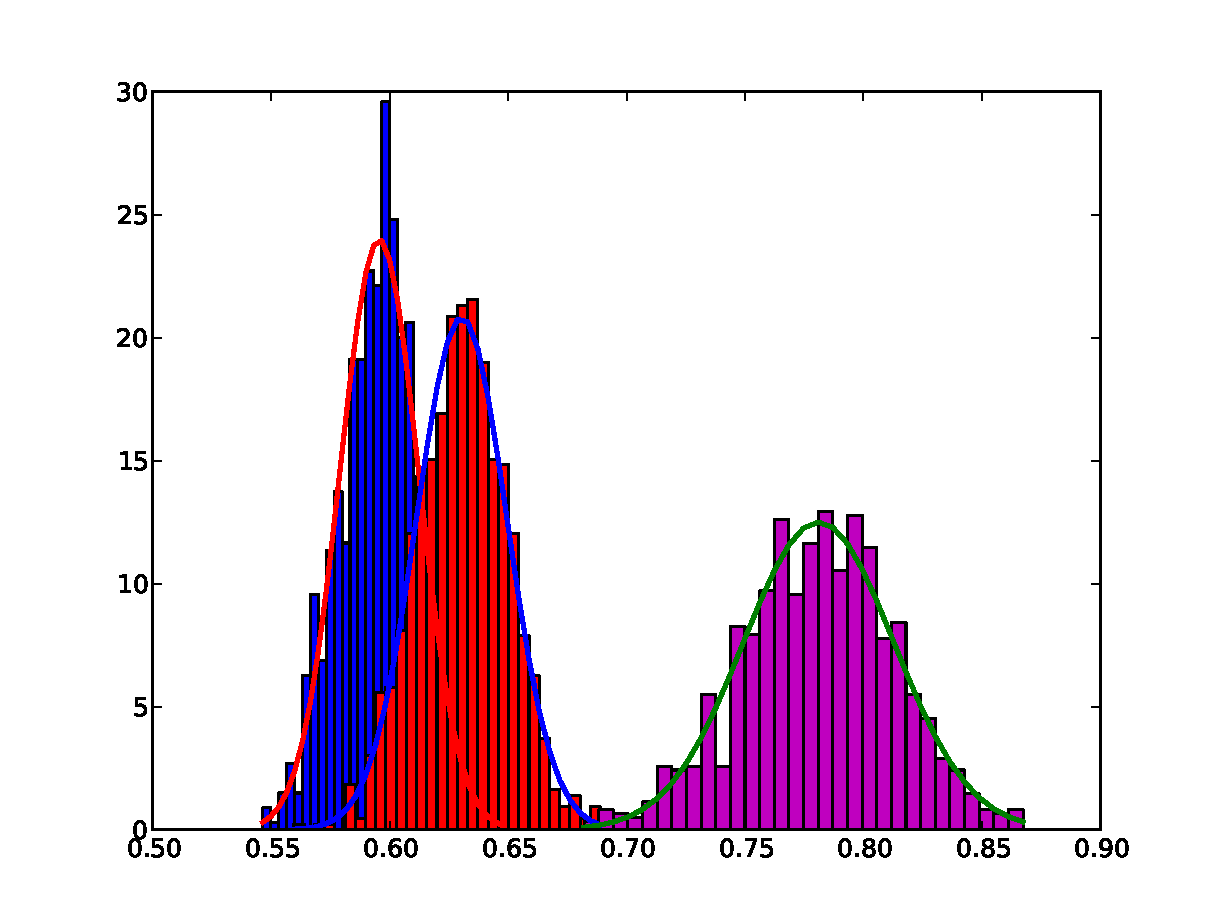
\includegraphics[width=0.8\textwidth]{three_classifiers.pdf}
    \caption{The accuracy of the three sentiment analysers is shown using their normal distributions calculated from the mean and standard deviation of their results. The blue bars indicate the accuracy of the Speculative word list, the red bars show the derived word list and the violet bars show the Na\"\i ve Bayes approach}
    \label{fig:three_classifiers}
    \end{center}
\end{figure}

In ~\ref{fig:three_classifiers} a Normal distribution is calculated from the mean and standard deviation the results to give the reader a visual aid as to where further tests accuracy results are likely to be for each classifier. From this graph it can be gathered that although there is a greater variance between in the accuracies of the Na\"\i ve Bayes classifier they are more far more likely to be greater than the results of word list based approaches. Although there is a considerable overlap in the speculative and derived word list's distributions the variance is much less, with the derived word list approach improving the speculative classifier on average. These results fail to nullify hypotheses ~\ref{hyp:h1} and ~\ref{hyp:h2}.

\subsection{The Effects of Changing Training Data Size}

The experiments regarding the changing of the training data set size took place on the Na\"\i ve Bayes Classifier first the 80\% split of training data was cut down to only 400 reviews before being increased to 1000 reviews before finally using the maximum training data provided by the 80\% split (1,600 reviews). These results are once again the mean average of domain specific experiments, the results are tabulated in the Table~\ref{tab:varying_table}.

\begin{table}
    \begin{center}
    \caption{Table displaying the mean accuracy for tests that took place with the Na\"\i ve Bayes classifier when trained on varying sizes of training data}
    \label{tab:varying_table}
    \begin{tabular}{| l | l | l |}
        \hline
        Training Set Size & Mean Accuracy & Std. Deviation \\ \hline
        400 Reviews & 0.5 & 0 \\ \hline
        1000 Reviews & 0.7417 & 0.03795 \\ \hline
        1600 Reviews & 0.7847 & 0.01782 \\ \hline
    \end{tabular}
    \end{center}
\end{table}

The results of limiting the training set to only 400 documents was very surprising as all tests resulted in an accuracy of 0.5. This particular experiment was run several times to verify it wasn't a mistake. The mean for this experiment therefore came to 0.5 with a standard deviation of one. As a training set of 400 reviews lead to an essentially random classification of documents only the mean values for 1000 and 1600 are compared in Figure ~\ref{fig:vary_comare}.

\begin{figure}
    \centering
    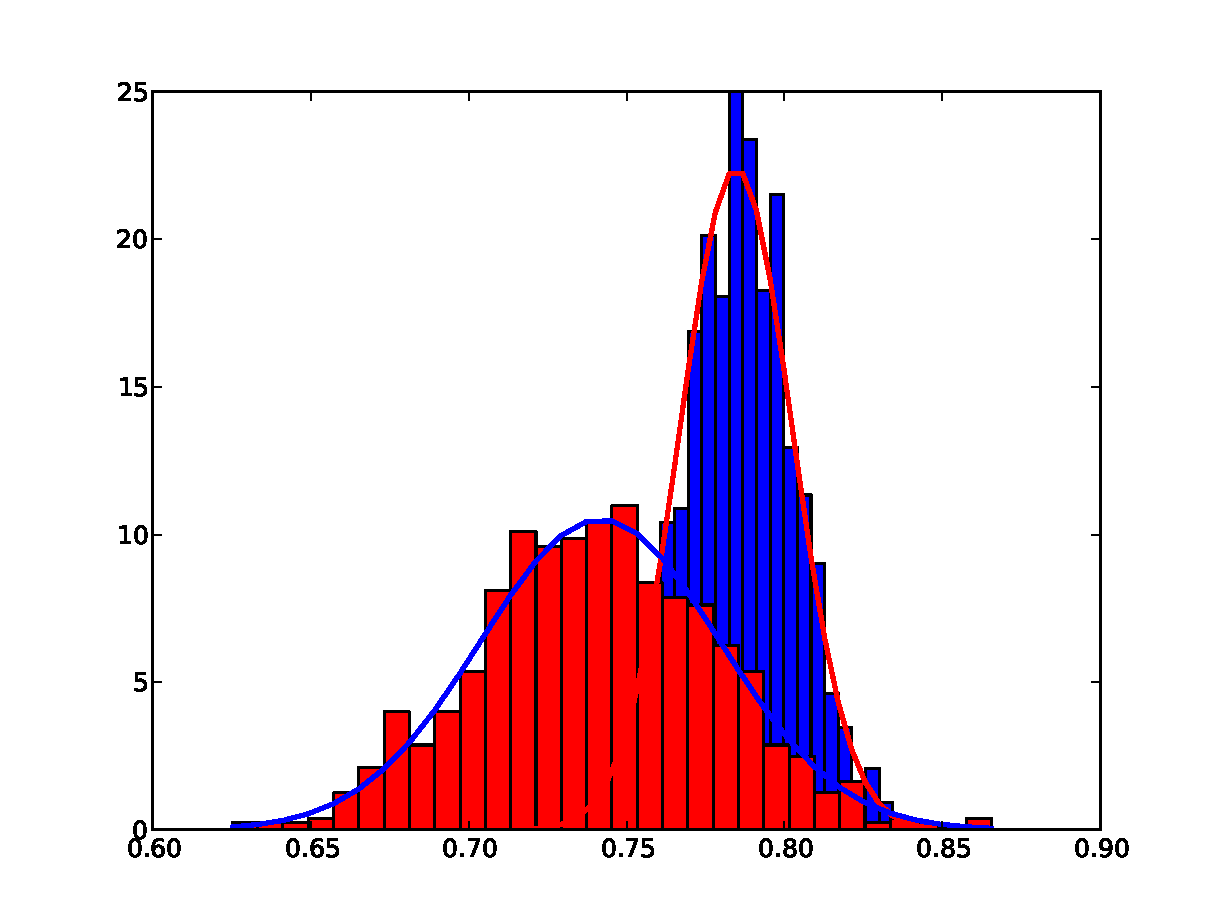
\includegraphics[width=0.8\textwidth]{vary_comparison.pdf}
    \caption{Naive Bayes' mean accuracy and standard deviation when training on 1600 reviews is shown in blue bars and a red line shown in the form of a normal distribution. 1000 reviews is shown with red bars and a blue line.}
    \label{fig:vary_comare}
\end{figure}

As is visible in Figure ~\ref{fig:vary_comare} the variance in accuracy is almost halved and the average accuracy increases when the training data set size jumps from 1000 to 1600 reviews. Although this is far from proved, it can be drawn from this conclusion or intuition that the larger the training data set the higher the accuracy of the trained classifier. Due to the experiments conditions, this notion assumes that the training data is of the same domain as the testing data. With this information alone ~\ref{hyp:h3} cannot be refuted.

\subsection{Na\"\i ve Bayes Cross-Domain Performance}
As the implementation for the experiments allowed for each domain to be tested separately by looping through a list of the Amazon review categories and testing a random 80\% split training with the testing data of the same domain a natural way to implement multiple cross domain tests was to save the testing set of first category in the loop and test every classifier trained on other domains against the first testing set's domain. In the following two experiments the domains books and electronics where held and tested on every other domain as well as themselves. The results and interesting comparisons are displayed in Figures ~\ref{fig:book_crossdomain}, ~\ref{fig:book_on_dvd}, ~\ref{fig:elec_crossdomain}, and ~\ref{fig:kitchen_on_elec}.

\begin{figure}
    \centering
    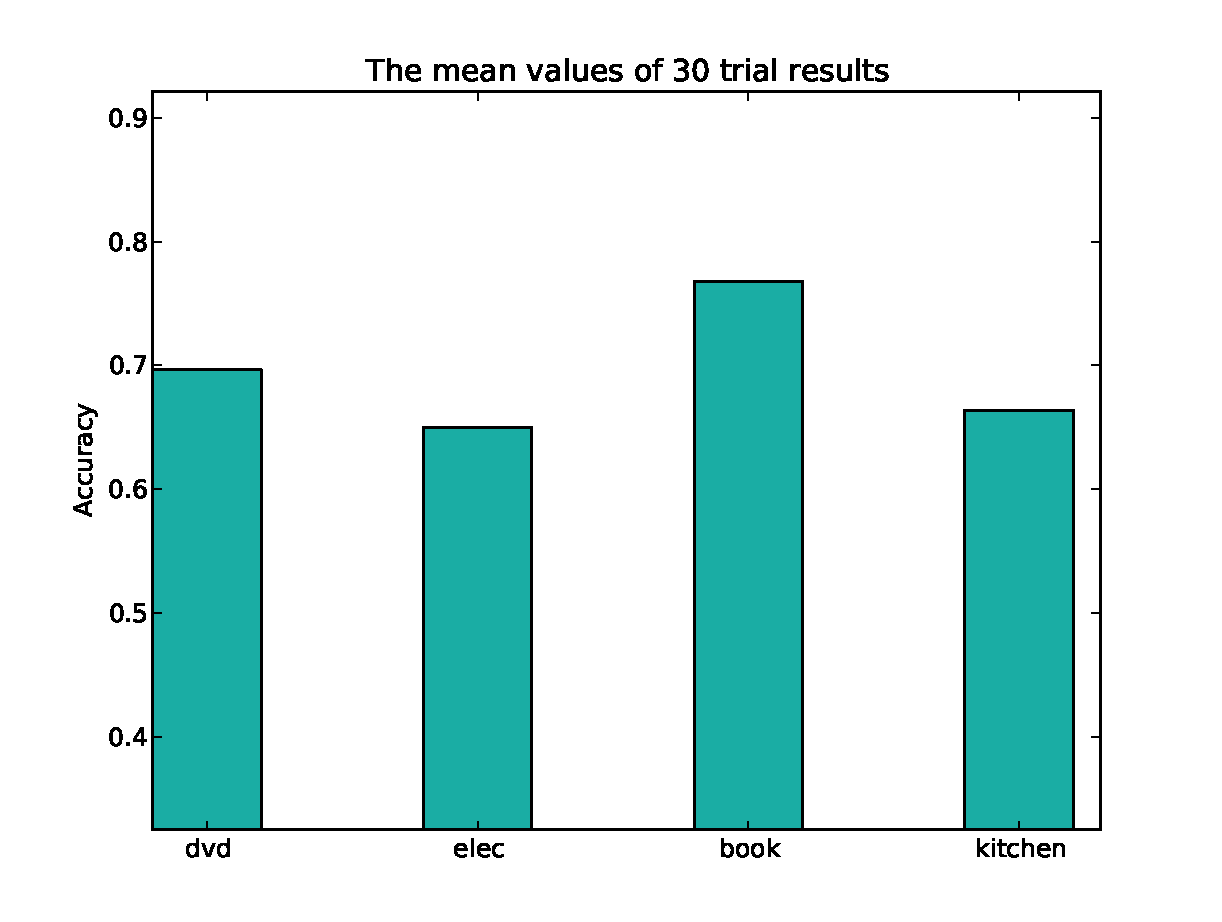
\includegraphics[width=0.8\textwidth]{crossdomain_book_nb.pdf}
    \caption{A bar chart depicting the average accuracy of the Na\"\i ve Bayes Classifier when trained on reviews of some domain and then tested on only book review data.}
    \label{fig:book_crossdomain}
\end{figure}

\begin{figure}
    \centering
    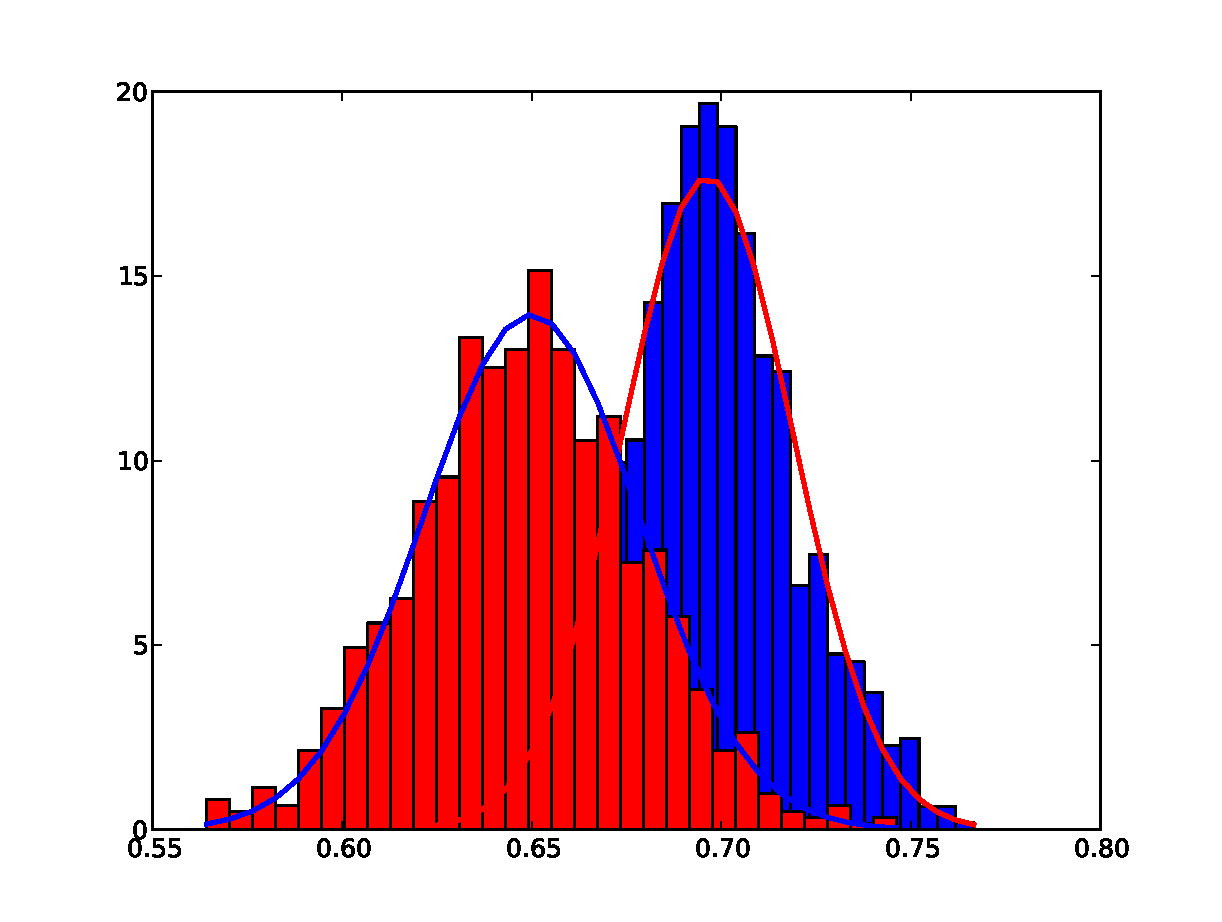
\includegraphics[width=0.8\textwidth]{crossdomain_book_nb_bookONdvd.pdf}
    \caption{Comparing the Na\"\i ve Bayes Classifier when trained on Books and DVD domains but tested on only Book review data. A normal distribution is shown using the average mean accuracy and the standard deviation of the results. Books are displayed with blue bars and a red line.}
    \label{fig:book_on_dvd}
\end{figure}

\begin{figure}
    \centering
    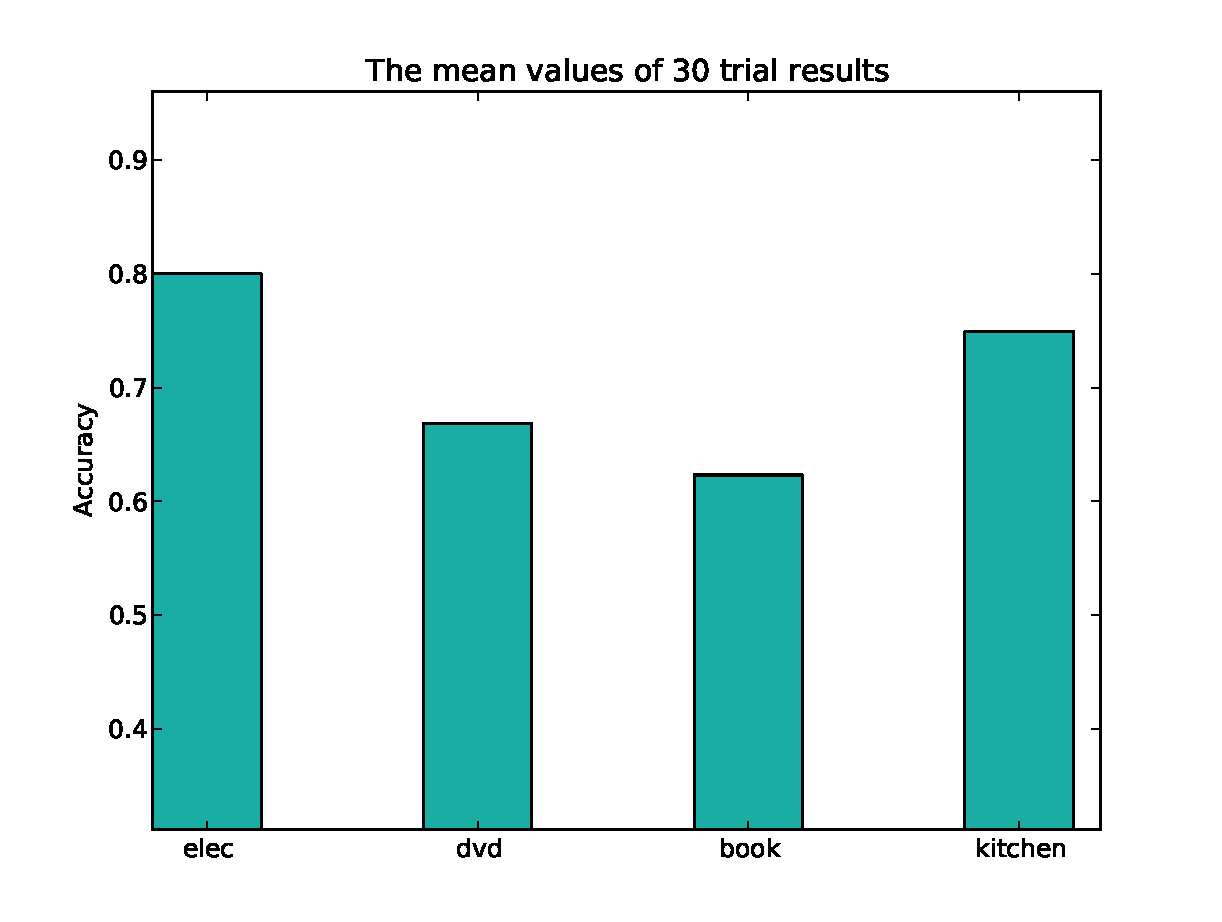
\includegraphics[width=0.8\textwidth]{crossdomain_elec_nb.pdf}
    \caption{A bar chart depicting the average accuracy of the Na\"\i ve Bayes Classifier when trained on reviews of some domain and then tested on only electronics review data.}
    \label{fig:elec_crossdomain}
\end{figure}

\begin{figure}[kit_on_elec]
    \centering
    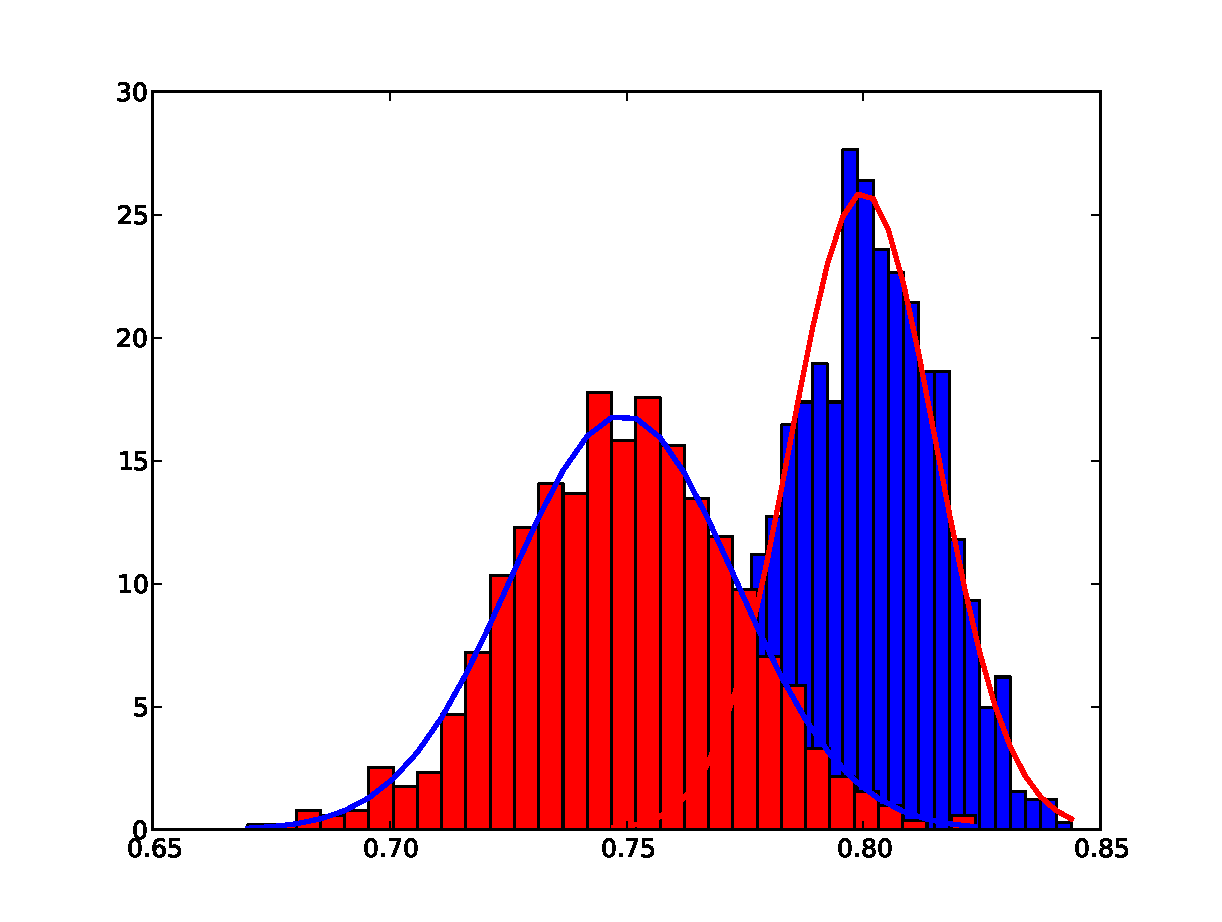
\includegraphics[width=0.8\textwidth]{crossdomain_elec_nb_kitchenONelec.pdf}
    \caption{Comparing the Na\"\i ve Bayes Classifier when trained on Kitchen and Electronics domains but tested on only Electronics review data. A normal distribution is shown using the average mean accuracy and the standard deviation of the results. Electronics are displayed with blue bars and a red line.}
    \label{fig:kitchen_on_elec}
\end{figure}

It is interesting to note that when book reviews are used as the testing data across domains that DVD's achieve the highest average accuracy after a classifier trained on the books domain. A possible reason for this may be because of the slight relation between the two categories, as both can be used as forms of relaxation, similar words may be used to describe them in a positive and negative light. A similar incident occurs when Electronics reviews are held as the testing set. When the cross domain results are looked at the Kitchen item reviews are the highest which may have something to do with many kitchen items being reviewed may have electrical parts and similar words are used to describe these items negatively such as `broken' and `faulty' which is less likely to apply to DVD and Books. However, these observations are strictly speculative and further statistical analysis would be needed on a larger data set in order to draw conclusions and to ensure these results are not just anomalies. In comparison to the cross domain testing results, when the classifier trains on the domain that it is tested on it performs significantly better which does not disprove \ref{hyp:h4}.

\subsection{Comparison of Feature Extraction Methods} % TODO
These experiments took three functions which processed and modified the data sets before being used with the Na\"\i ve Bayes classifier. The first function removes all uppercase characters and replaces them with lowercase characters. The second replaces all numerical tokens with the string `NUM' and the final feature extracting function removes any occurrence of a word from a list of stop words provided by the NLTK library. The mean accuracies are graphed in the following Figures ~\ref{fig:fe_nofe}, ~\ref{fig:fe_lowercase}, ~\ref{fig:fe_num}, ~\ref{fig:fe_stopwords}.

\begin{figure}
    \centering
    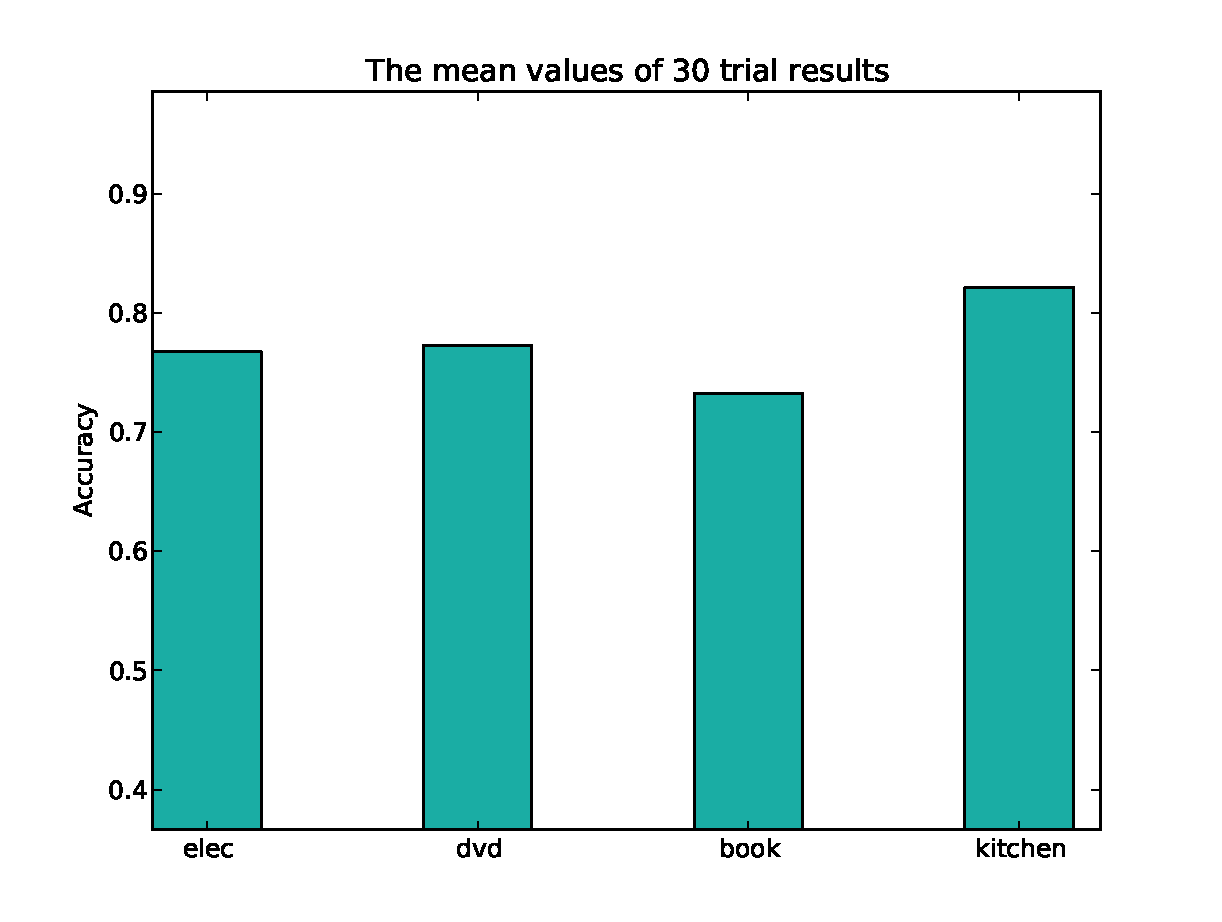
\includegraphics[width=0.8\textwidth]{nb_no_feature_extractor.pdf}
    \caption{This bar chart shows the mean accuracy for the Na\"\i ve Bayes classifier for each separate domain when no feature extraction techniques are applied.}
    \label{fig:fe_nofe}
\end{figure}

\begin{figure}
    \centering
    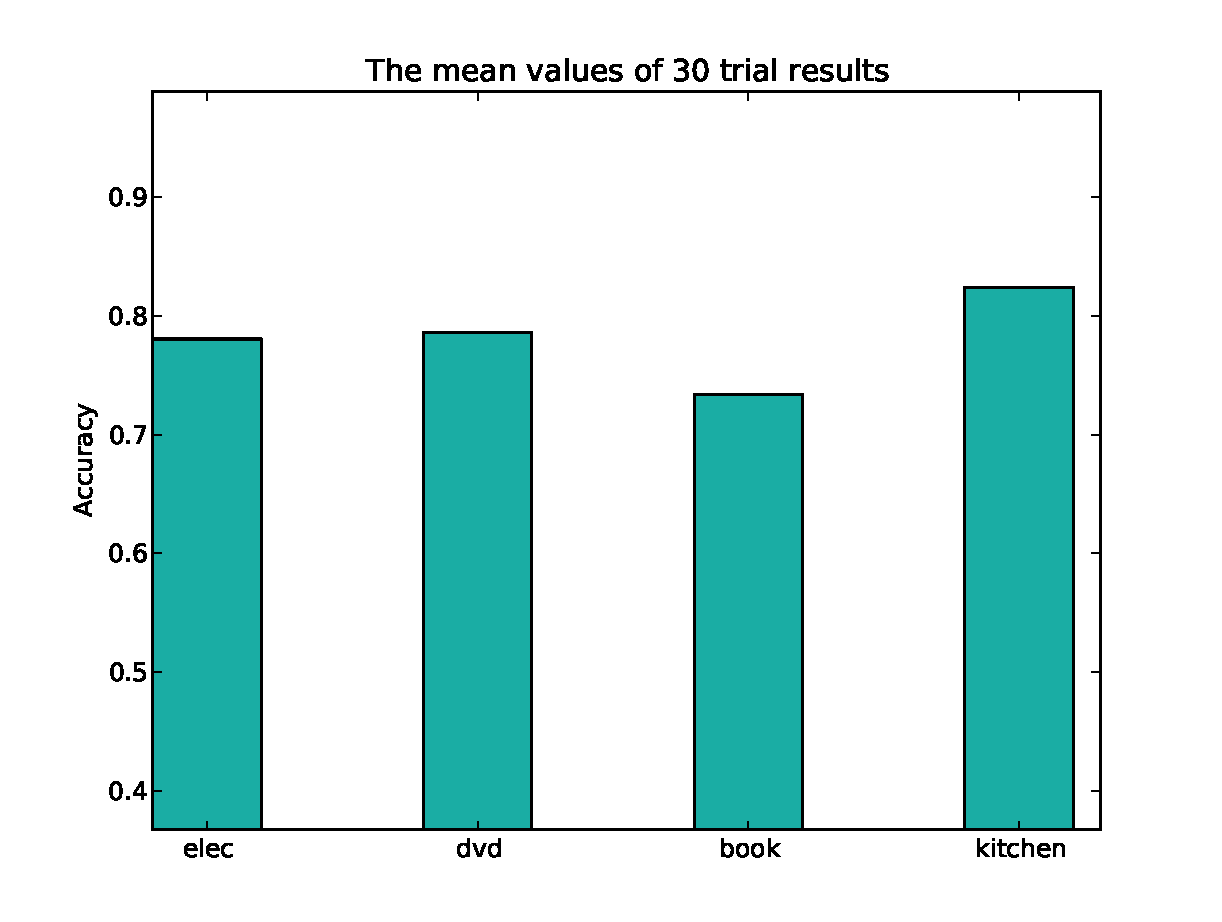
\includegraphics[width=0.8\textwidth]{nb_feature_extractor_lowercase.pdf}
    \caption{This bar chart shows the mean accuracy for the Na\"\i ve Bayes classifier for each separate domain when uppercase characters are removed from both training and testing data and replaced with lowercase characters.}
    \label{fig:fe_lowercase}
\end{figure}

\begin{figure}
    \centering
    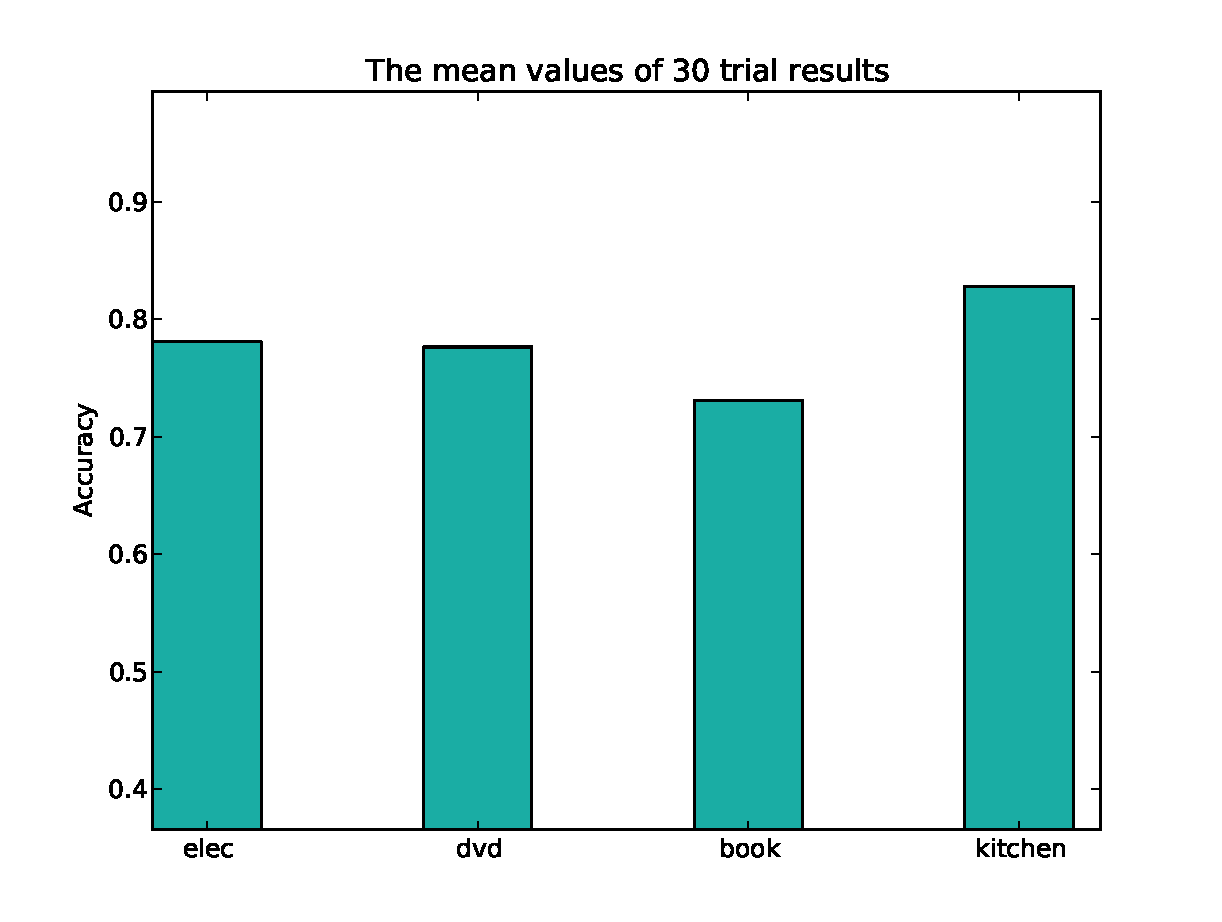
\includegraphics[width=0.8\textwidth]{nb_feature_extractor_num.pdf}
    \caption{This bar chart shows the mean accuracy for the Na\"\i ve Bayes classifier for each separate domain when both uppercase characters are removed and all numbers are replaced with the string `NUM'.}
    \label{fig:fe_num}
\end{figure}

\begin{figure}
    \centering
    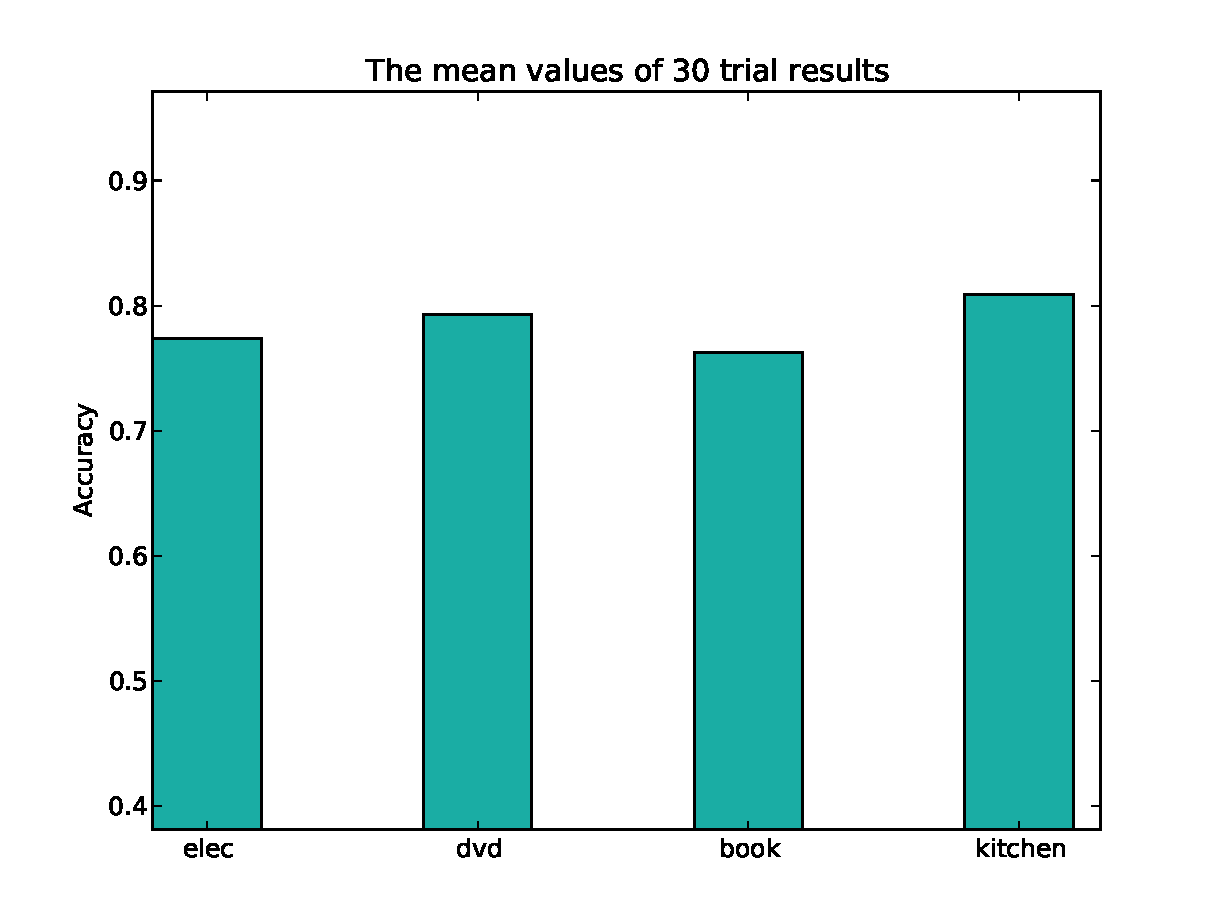
\includegraphics[width=0.8\textwidth]{nb_feature_extractor_stopwords.pdf}
    \caption{This bar chart shows the mean accuracy for the Na\"\i ve Bayes classifier for each separate domain when uppercase characters and numbers are replaced as well as all words on NLTK's stop words being removed}
    \label{fig:fe_stopwords}
\end{figure}

These figures show a large initial increase in the accuracy of the classifier as more feature extractors are added. It appears that the application of the `lowercase' feature extractor produced the greatest increase in the average accuracy of the classifier but the rate of change in accuracy to further feature extraction tails off almost immediately. This finding disproves \ref{hyp:h5} as the addition of further feature extraction techniques does not necessarily improve the accuracy of Na\"\i ve Bayes classifiers. The size of the initial increase in accuracy could be due to the fact that it was the first feature extraction method to be added to the stack. Further tests should be carried out in order to determine whether or not the lowercase feature extraction method is the most effective in improving the accuracy of the classifier. Another useful point to note is the noticeable performance impact the stop words feature extractor made on the experiments while making the most marginal increases in accuracy.

\subsection{Informative Features}

The final analysis of the Na\"\i ve Bayes classifier with the score based classifiers looks at what the NLTK library, which provides the Na\"\i ve Bayes implementation used in these experiments, calls `most informative features'. The top ten positive and negative words used by the derived word list approach are tabulated below for each domain, followed by the most informative words lists from NLTK for each domain. There are many interesting points that can be made when making comparisons between the word lists of all classifiers.

\begin{center}
    \begin{table}
    \caption{Derived Word list post- stop words 100 most frequent words (Electronics - top 10)}
    \begin{minipage}{.5\linewidth}
    \caption{}
    \centering
    \begin{tabular}{| l |}
        \hline
        Positive Words \\ \hline
        'NUM' \\ \hline
        'one' \\ \hline
        'use' \\ \hline
        'great' \\ \hline
        'good' \\ \hline
        'sound' \\ \hline
        'would' \\ \hline
        'like' \\ \hline
        'quality' \\ \hline
        'price' \\ \hline
    \end{tabular}
    \end{minipage}%
    \begin{minipage}{.5\linewidth}
    \centering
    \caption{}
    \begin{tabular}{| l |}
        \hline
        Negative Words \\ \hline
        'NUM' \\ \hline
        'one' \\ \hline
        'would' \\ \hline
        'get' \\ \hline
        'work' \\ \hline
        'use' \\ \hline
        'product' \\ \hline
        'bought' \\ \hline
        'back' \\ \hline
        'time' \\ \hline
    \end{tabular}
    \end{minipage} 
    \end{table}
\end{center}


\begin{center}
    \begin{table}
    \caption{Derived Word list post- stop words 100 most frequent words (DVD - top 10)}
    \begin{minipage}{.5\linewidth}
    \caption{}
    \centering
    \begin{tabular}{| l |}
        \hline
        Positive Words \\ \hline
        'NUM' \\ \hline
        'film' \\ \hline
        'movie' \\ \hline
        'one' \\ \hline
        'great' \\ \hline
        'like' \\ \hline
        'dvd' \\ \hline
        'good' \\ \hline
        'well' \\ \hline
        'first' \\ \hline
    \end{tabular}
    \end{minipage}%
    \begin{minipage}{.5\linewidth}
    \centering
    \caption{}
    \begin{tabular}{| l |}
        \hline
        Negative Words \\ \hline
        'movie' \\ \hline
        'NUM' \\ \hline
        'film' \\ \hline
        'one' \\ \hline
        'like' \\ \hline
        'dvd' \\ \hline
        'would' \\ \hline
        'good' \\ \hline
        'even' \\ \hline
        'get' \\ \hline
    \end{tabular}
    \end{minipage} 
    \end{table}
\end{center}


\begin{center}
    \begin{table}
    \caption{Derived Word list post- stop words 100 most frequent words (Books - top 10)}
    \begin{minipage}{.5\linewidth}
    \caption{}
    \centering
    \begin{tabular}{| l |}
        \hline
        Positive Words \\ \hline
        'book'\\ \hline
        'one'\\ \hline
        'NUM'\\ \hline
        'read'\\ \hline
        'would'\\ \hline
        'like'\\ \hline
        'time'\\ \hline
        'story'\\ \hline
        'many'\\ \hline
        'also'\\ \hline
    \end{tabular}
    \end{minipage}%
    \begin{minipage}{.5\linewidth}
    \centering
    \caption{}
    \begin{tabular}{| l |}
        \hline
        Negative Words \\ \hline
        'book' \\ \hline
        'NUM' \\ \hline
        'one' \\ \hline
        'read' \\ \hline
        'like' \\ \hline
        'would' \\ \hline
        'much' \\ \hline
        'books' \\ \hline
        'even' \\ \hline
        'good' \\ \hline
    \end{tabular}
    \end{minipage} 
    \end{table}
\end{center}

\begin{center}
    \begin{table}
    \caption{Derived Word list post- stop words using 100 most frequent words (Kitchen - top 10)}
    \begin{minipage}{.5\linewidth}
    \caption{}
    \centering
    \begin{tabular}{| l |}
        \hline
        Positive Words \\ \hline
        'NUM' \\ \hline
        'use' \\ \hline
        'one' \\ \hline
        'great' \\ \hline
        'like' \\ \hline
        'easy' \\ \hline
        'well' \\ \hline
        'would' \\ \hline
        'love' \\ \hline
        'pan' \\ \hline
    \end{tabular}
    \end{minipage}%
    \begin{minipage}{.5\linewidth}
    \centering
    \caption{}
    \begin{tabular}{| l |}
        \hline
        Negative Words \\ \hline
        'NUM'\\ \hline
        'one'\\ \hline
        'would'\\ \hline
        'use'\\ \hline
        'time'\\ \hline
        'get'\\ \hline
        'coffee'\\ \hline
        'like'\\ \hline
        'product'\\ \hline
        'even'\\ \hline
    \end{tabular}
    \end{minipage} 
    \end{table}
\end{center}


\begin{center}
    \begin{table}
    \caption{Na\"\i ve Bayes Bayes Most Informative Words post- stop words}
    \begin{minipage}{.5\linewidth}
    \caption{(Electronics - top 10)}
    \centering
    \begin{tabular}{| l | l |}
        \hline
        Word & Sentiment \\ \hline
        refund & Negative \\ \hline
        return & Negative \\ \hline
        terrible & Negative \\ \hline
        waste & Negative \\ \hline
        junk & Negative \\ \hline
        worst & Negative \\ \hline
        contacted & Negative \\ \hline
        provides & Positive \\ \hline
        stopped & Negative \\ \hline
        beware & Negative \\ \hline
    \end{tabular}
    \end{minipage}%
    \begin{minipage}{.5\linewidth}
    \centering
    \caption{(DVD - top 10)}
    \begin{tabular}{| l | l |}
        \hline
        Word & Sentiment \\ \hline
        waste & Negative \\ \hline
        ridiculous & Negative \\ \hline
        awful & Negative \\ \hline
        lame & Negative \\ \hline
        terrific & Positive \\ \hline
        poorly & Negative \\ \hline
        dumb & Negative \\ \hline
        paid & Negative \\ \hline
        crap & Negative \\ \hline
        smart & Positive \\ \hline
    \end{tabular}
    \end{minipage} 
    \end{table}
\end{center}


\begin{center}
    \begin{table}
    \caption{Na\"\i ve Bayes Bayes Most Informative Words post- stop words}
    \begin{minipage}{.5\linewidth}
    \caption{Book - top 10}
    \centering
    \begin{tabular}{| l | l |}
        \hline
        Words & Sentiment \\ \hline
        disappointing & Negative \\ \hline
        poorly & Negative \\ \hline
        waste & Negative \\ \hline
        devoted & Negative \\ \hline
        useless & Negative \\ \hline
        flat & Negative \\ \hline
        boring & Negative \\ \hline
        superficial & Negative \\ \hline
        endless & Negative \\ \hline
        subsequent & Positive \\ \hline
    \end{tabular}
    \end{minipage}%
    \begin{minipage}{.5\linewidth}
    \centering
    \caption{Kitchen - top 10}
    \begin{tabular}{| l | l |}
        \hline
        Words & Sentiment \\ \hline
        worst & Negative \\ \hline
        returned & Negative \\ \hline
        junk & Negative \\ \hline
        refund & Negative \\ \hline
        unfortunately & Negative \\ \hline
        favorite & Positive \\ \hline
        loves & Positive \\ \hline
        told & Negative \\ \hline
        everywhere & Negative \\ \hline
        followed & Negative \\ \hline
    \end{tabular}
    \end{minipage} 
    \end{table}
\end{center}

One interesting point to raise is the amount of words that may be perceived as positive or neutral to the human eye that appear in the derived words list's top ten negative words list across all domains. The majority of words that appear in the derived word list's top ten for either positive or negative do not appear in either the speculative word list or the Na\"\i ve Bayes' most informative features. The domain that the classifier is also very effective on the most informative features of the classifier with words like `endless' for a negative book review or `beware' for a negative electronics review. Finally it is worth mentioning that there are many negative words produced by the Na\"\i ve Bayes it could be reasoned that negative words appear less in positive documents. The probability positive words like `good' being present in a document and influencing the classification is weakened by the fact that positive words are more likely to occur in negative documents after a negation, for example, `no good' or `not great'.

\section{Further Work}

There are certain features, factors and methods that this paper would have benifited from exploring but due to time constraints this was not possible. Cross validation through the use of k-folding would have been a better approach to use in carrying out these experiments as the method ensures all reviews are used for both training and testing, and each review is only used for testing once. Furthering this, if the splits and the data contained in each split remains constant between the testing of different classifiers the tests can be compared fairly.

\section{Conclusion}
In this paper five hypotheses were put forward and small experiments were carried out in order to test them. Multiple document classification methods were explained and used against the Amazon Review Corpus which was prepared by the Text Analytics Group at the University of Sussex. The results of these were analysed leading to only one of the hypotheses being disproved, but better testing methods could be used in order to ensure that these results were not an anomaly. The Na\"\i ve Bayes classifier produced some of the best accuracy results out of the classifiers that were analysed and looking at the words that it thought were most informative, compared to the other word list based approaches, the Na\"\i ve Bayes classifier appears more sophisticated. Even though the results in this paper draw lead to these conclusions it does not neccessarily mean that these assumptions maybe applied across different corpora.

%The bibliography, done here without a bib file
%This is the old BibTeX style for use with llncs.cls
\bibliographystyle{splncs}

%Alternative bibliography styles:
%the following does the same as above except with alphabetic sorting
%\bibliographystyle{splncs_srt}
%the following is the current LNCS BibTex with alphabetic sorting
%\bibliographystyle{splncs03}
%If you want to use a different BibTex style include [oribibl] in the document class line

\begin{thebibliography}{1}
%add each reference in here like this:
\bibitem[WD1]{Weir2013}
Weir, D.
Lecture Notes
(2013)
\end{thebibliography}

\end{document}

